\section{Evaluation}
\label{sec:evaluation}
In this section, we evaluate \sys under different sizes of LLMs ranging from 13B to 175B and various application datasets including chatbot, code-completion, and summarization. The evaluation shows that \sys consistently outperforms the current state-of-the-art system across all the settings (\S\ref{exp:end_to_end}). Specifically, \sys can handle up to $7.4\times$ higher rates and $12.6\times$ more stringent SLO while meeting the latency requirements for over 90\% requests. Additionally, we analyze the latency breakdown in \sys to show the communication overhead is insubstantial thanks to our bandwidth-aware placement algorithm (\S\ref{exp:breakdown}) and do ablation studies of our techniques (\S\ref{exp:ablation}). Finally, we profile the execution time of our placement algorithm (\S\ref{exp:run_time}).

\begin{table}[t]
    \centering
    \resizebox{1\linewidth}{!} {
    \begin{tabular}{ccccc}
        \toprule
        \textbf{Application} & \textbf{Model Size} & \textbf{TTFT} & \textbf{TPOT} & \textbf{Dataset} \\
        \midrule
        Chatbot OPT-13B & 26GB & 0.25s & 0.1s & ShareGPT~\cite{sharegpt} \\
        Chatbot OPT-66B & 132GB & 2.5s & 0.15s & ShareGPT~\cite{sharegpt} \\
        Chatbot OPT-175B & 350GB & 4.0s & 0.2s & ShareGPT~\cite{sharegpt} \\
        Code Completion OPT-66B & 132GB & 0.125s & 0.2s & HumanEval~\cite{chen2021codex} \\
        Summarization OPT-66B & 132GB & 15s & 0.15s & LongBench~\cite{bai2023longbench} \\
        \bottomrule
    \end{tabular}
    }
    \caption{Workloads in evaluation and latency requirements.}
    \label{tab:app_config}
\end{table}

\begin{figure}[!t]
    \centering
    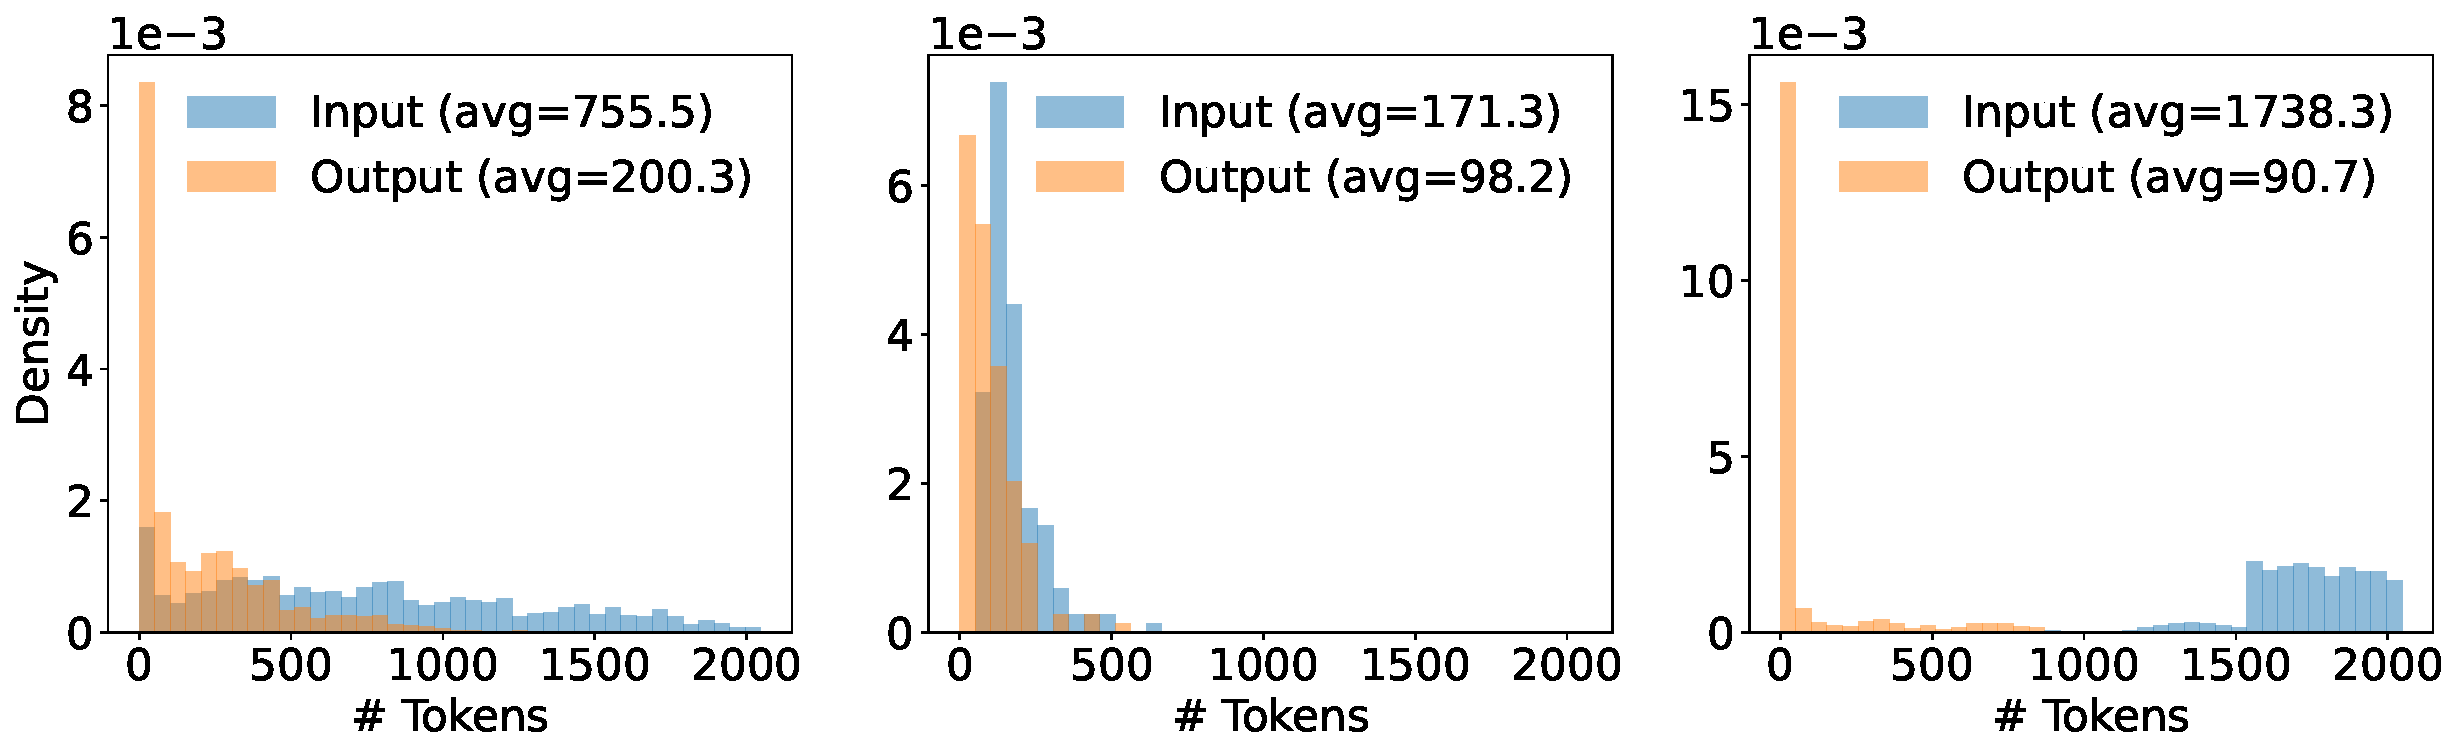
\includegraphics[width=\linewidth]{figures/evaluation/dataset.pdf}
    (a) ShareGPT \hspace{8mm} (b) HumanEval \hspace{8mm} (c) LongBench
    \caption{The input and output length distributions of (a) ShareGPT, (b) HumanEval, and (c) LongBench datasets.}
    \vspace{-4mm}
    \label{fig:dataset}
\end{figure}

\begin{figure*}[!t]
    \centering
    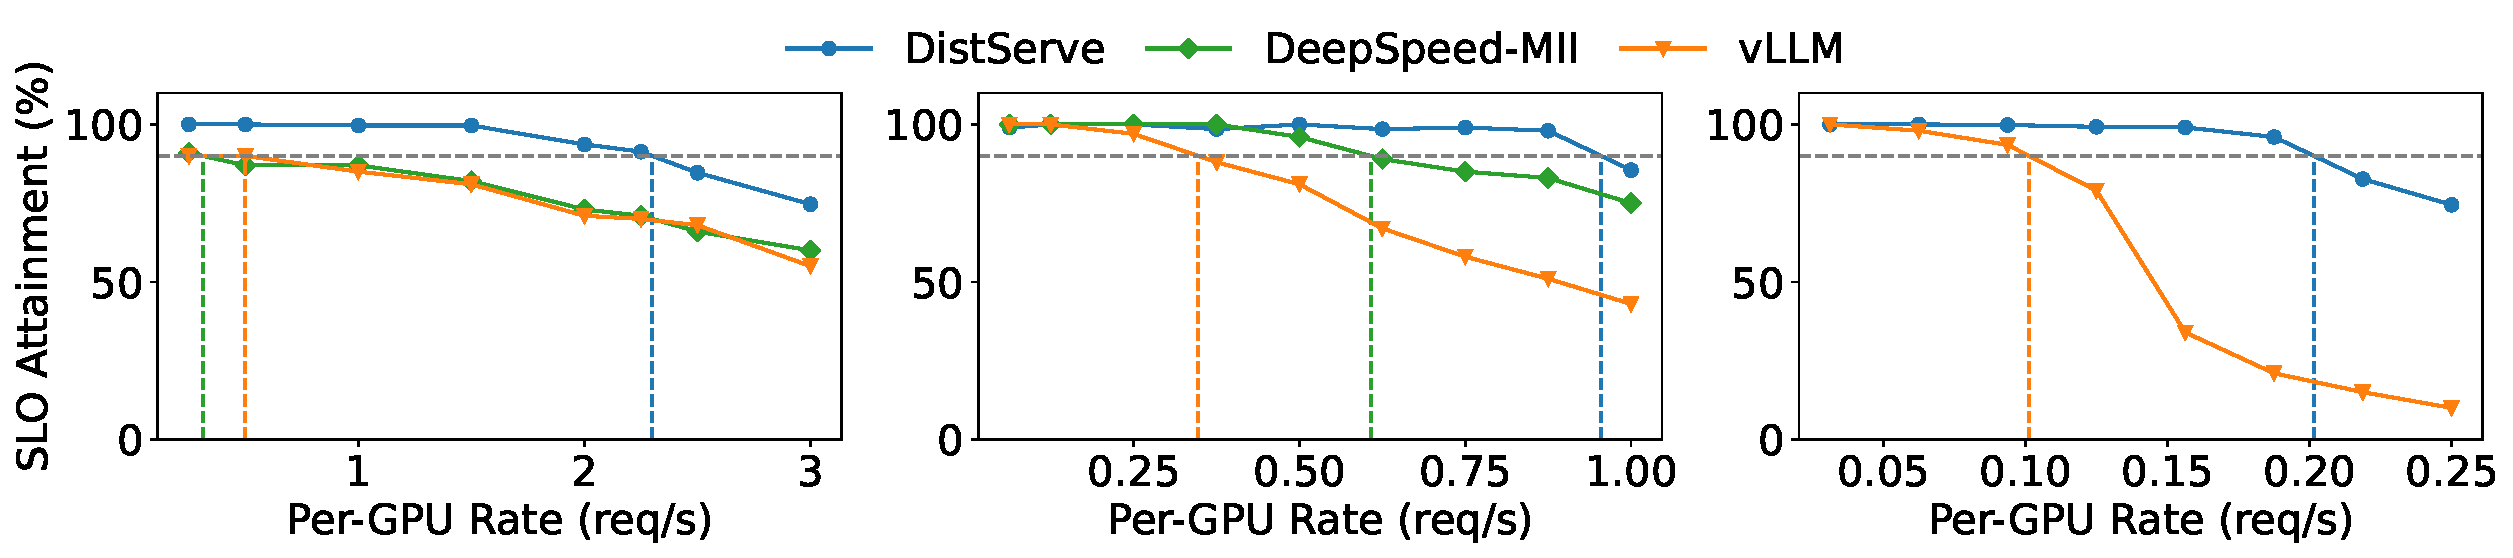
\includegraphics[width=0.95\linewidth]{figures/evaluation/chatbot-rate-p90.pdf}
    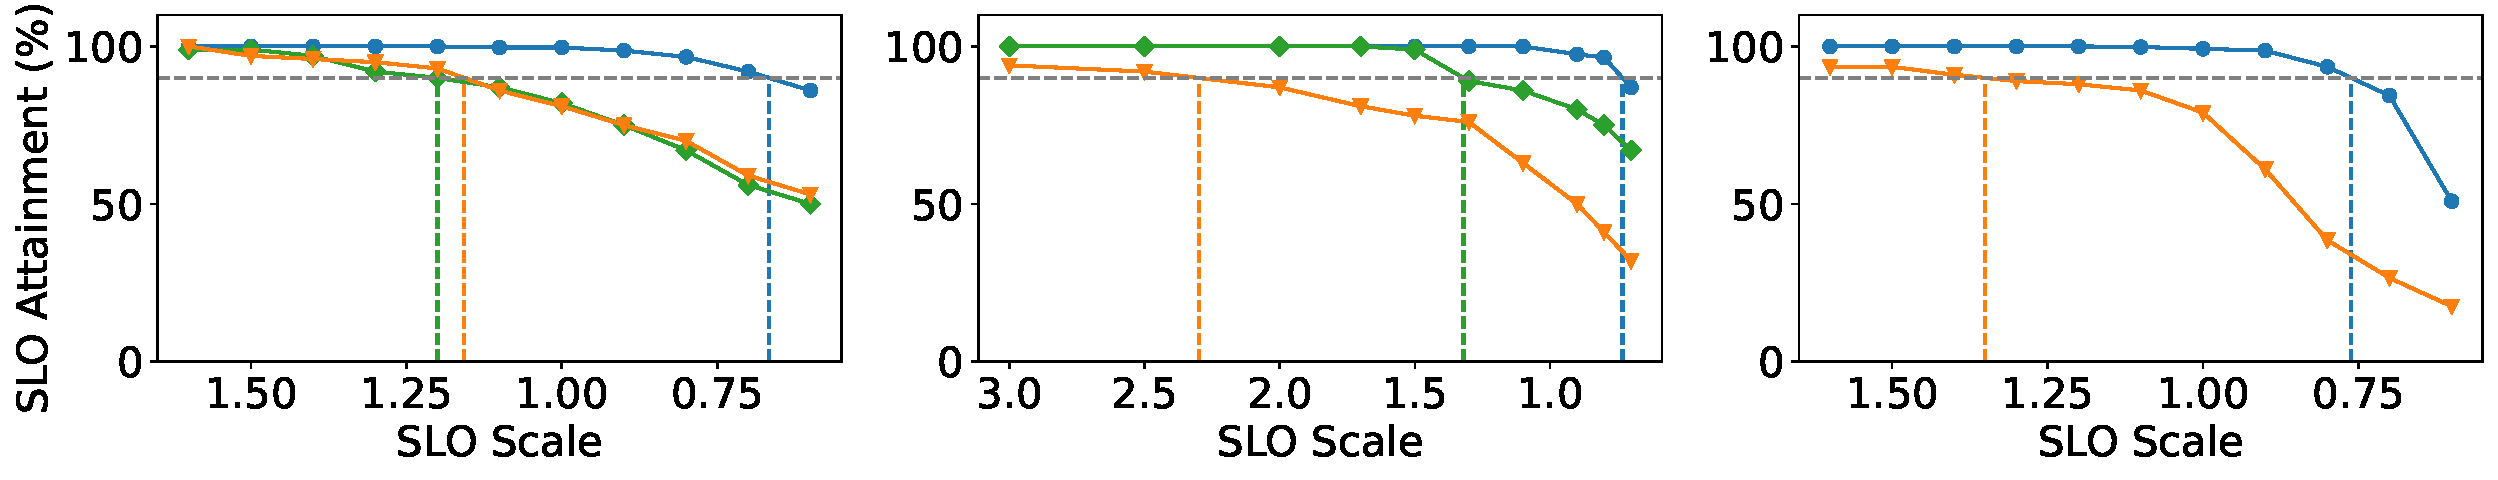
\includegraphics[width=0.95\linewidth]{figures/evaluation/chatbot-SLO-p90.pdf}
    \hspace{10mm} (a) OPT-13B \hspace{40mm} (b) OPT-66B \hspace{40mm} (C) OPT-175B
    \caption{Chatbot application with OPT models on the ShareGPT dataset.}
    \vspace{-4mm}
    \label{fig:chatbot}
\end{figure*}

\subsection{Experiments Setup}
\paraf{Cluster testbed.} We deploy \sys on a cluster with 4 nodes and 32 GPUs. Each node has 8 NVIDIA SXM A100-80GB GPUs connected with NVLINK. The cross-node bandwidth is 25Gbps. Due to the limited cross-node bandwidth, we use the low node-affinity placement algorithm (\S\ref{alg:low-affinity-placement}) for \sys in most of the experiments except for the ablation study (\S\ref{exp:ablation}) which uses simulation.

\parabf{Model and workloads setup.} Similar to prior work on LLM serving~\cite{vllm}, we choose the OPT~\cite{zhang2022opt} model series, which is a representative LLM family widely used in academia and industry. Newer GPT model families are adopting memory-efficient attention mechanisms like GQA~\cite{ainslie2023gqa} and MQA~\cite{mqa}. \sys will show better performance on these models because the transmission overhead is lower due to the decrease in KV cache size. We choose OPT which uses the classic MHA~\cite{vaswani2017attention} to put enough pressure on the transmission overhead. We use FP16 precision in all experiments. For workloads, as shown in Table~\ref{tab:app_config}, We choose three typical LLM applications and set the SLOs empirically based on their service target because there exists no available SLO settings for these applications as far as we know. For each application, we select a suitable dataset and sample requests from it for evaluation. Since all the datasets do not include timestamps, we generate request arrival times using Poisson distribution with different request rates. Due to the space limit, we test the chatbot workload on all three OPT models and the other two workloads on OPT-66B, which matches the largest size in the recent open-source LLM series~\cite{touvron2023llama}.
\begin{itemize}[leftmargin=*]
    \item \textbf{Chatbot}~\cite{chatgpt}: We use the ShareGPT dataset~\cite{sharegpt} for the chatbot application, which is a collection of user-shared conversations with ChatGPT. For OPT-13B, the TTFT SLO is set to 0.25s for responsiveness and the TPOT SLO is set to 0.1s which is higher than the normal human read speed. For OPT-66B and OPT-175B, we slightly relax the two SLOs due to the increase in model execution latency. 
    \item \textbf{Code completion}~\cite{chen2021codex}: We use the HumanEval~\cite{chen2021codex} dataset for the code completion task. It includes 164 programming problems with a function signature or docstring which is used to evaluate the performance of code completion models. Since the code completion model is used as a personal real-time coding assistant, we set both SLOs to be stringent.
    \item \textbf{Summarization}~\cite{lanchain}: It is a popular LLM task to generate a concise summary for a long article, essay, or even an academic paper. We use LongBench~\cite{bai2023longbench} dataset which contains the summarization task\footnote{We capped the input lengths in LongBench because OPT’s absolute positional embedding only supports a maximum length of 2048.}. As shown in Figure~\ref{fig:dataset}, LongBench has much longer input lengths than the other two datasets. So we set a loose TTFT SLO but require a stringent TPOT.
\end{itemize}


\parabf{Metrics.} We use \textit{SLO attainment} as the major evaluation metric. Under a specific SLO attainment goal (say, 90\%), we are concerned with two things: the maximum per-GPU goodput and the minimal SLO the system can handle. We are particularly interested in an SLO attainment of 90\% (indicated by the vertical lines in all curve plots), but will also vary the rate and latency requirements to observe how the SLO attainment changes. We also include the results in the Appendix for an SLO attainment of 99\% to show the system performance under a more stringent SLO attainment target.

\parabf{Baselines.} We compare \sys to two baseline systems:

\begin{itemize}[leftmargin=*]
    \item \textbf{vLLM~\cite{vllm}:} vLLM is a representative LLM serving system widely used in both academia and industry. It supports \textit{continuous batching}~\cite{yu2022orca} to increase throughput and \textit{paged-attention}~\cite{vllm} to reduce memory fragmentation during KV cache allocation. However, it colocates the prefill and decoding computation to maximize the overall system throughput and struggles to meet the latency requirements cost-efficiently. Since vLLM only supports intra-op parallelism, we follow previous work~\cite{vllm} to set intra-op equals 1, 4, and 8 for the three OPT models, respectively.
    \vspace{2mm}
    \item \textbf{DeepSpeed-MII~\cite{deepspeed_mii}:} DeepSpeed Model Implementations for Inference (MII) supports \textit{chunked-prefill} by decomposing long prompts into smaller chunks and composing with short prompts to exactly fill a target token budget. It mitigates but cannot eliminate the prefill-decoding interference caused by the long prefill job. We set its intra-op the same as vLLM for OPT-13B and OPT-66B for a fair comparison. However, DeepSpeed-MII cannot serve OPT-175B whose $vocab\_size=50272$ because its underlying kernel implementation requires $vocab\_size/intra\_op$ is a multiple of 8 where intra-op equals 8 does not satisfy. Setting intra-op equals 4 can satisfy this requirement but will cause the out-of-memory issue.
\end{itemize}


\begin{figure*}[!t]
    \centering
    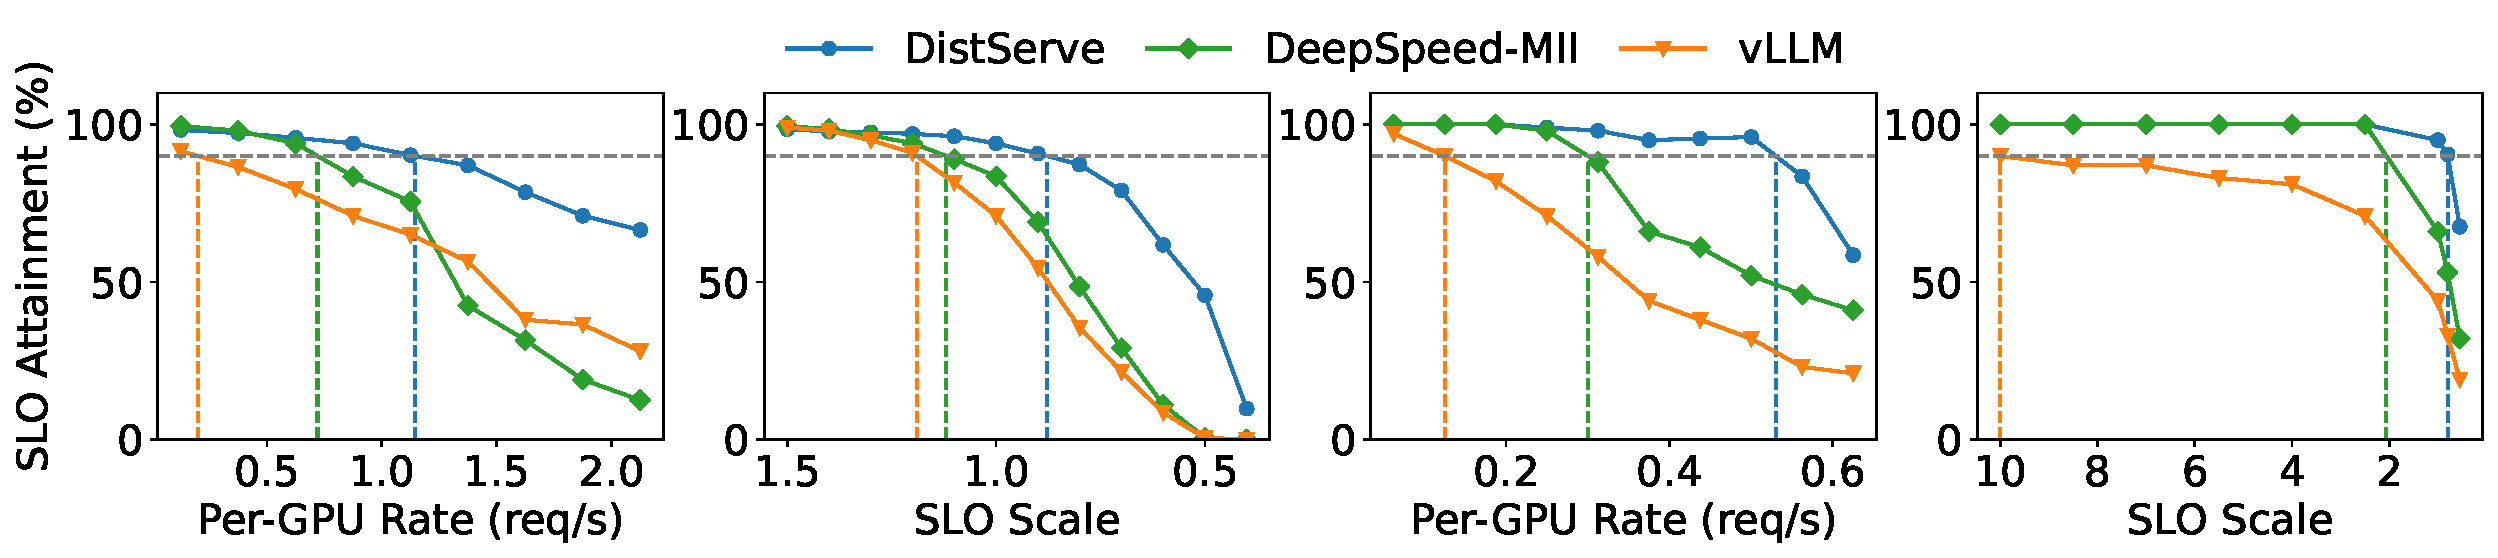
\includegraphics[width=0.95\linewidth]{figures/evaluation/other-apps-p90.pdf}
    \hspace{10mm} (a) Code Completion \hspace{50mm} (b) Summarization
    \caption{Code completion and summarization tasks with OPT-66B on HumanEval and LongBench datasets, respectively.}
    \vspace{-4mm}
    \label{fig:other_apps}
\end{figure*}

\subsection{End-to-end Experiments}
\label{exp:end_to_end}
In this Section, we compare the end-to-end performance of \sys against the baselines on real application datasets.

\parabf{Chatbot.} We evaluate the performance of \sys on the chatbot application for all three OPT models. The first row of Figure~\ref{fig:chatbot} illustrates that when we gradually increase the rate, more requests will violate the latency requirements and the SLO attainment decreases. The vertical line shows the maximum per-GPU rate the system can handle to meet latency requirements for over 90\% of the requests.

On the ShareGPT dataset, \sys can sustain $2.0\times$--$4.6\times$ higher request rate compared to vLLM. This is because DistLLM eliminates the prefill-decoding interference through disaggregation. Two phases can optimize their own objectives by allocating different resources and employing tailored parallelism strategies. Specifically, by analyzing the chosen placement strategy\footnote{All the placements chosen by \sys can be found in Appendix~\ref{appendix:placement_strategies}.} for 175B, we find the prefill instance has inter-op = 3, intra-op = 3; and the decoding instance has inter-op = 3, intra-op = 4. Under this placement, \sys can effectively balance the load between the two instances on ShareGPT, meeting latency requirements at the lowest cost. This non-trivial placement strategy is challenging to manually find, proving the effectiveness of the algorithm. In the case of vLLM, collocating prefill and decoding greatly slows down the decoding phase, thereby significantly increasing TPOT. Due to the stringent TPOT requirements of chatbot applications, although vLLM meets the TTFT SLO for most requests, the overall SLO attainment is dragged down by a large number of requests that violate the TPOT SLO. Compared to DeepSpeed-MII, \sys can sustain $1.6\times$--$7.4\times$ higher request rate. DeepSpeed-MII shows better performance on larger models because the prefill job is larger and chunked-prefill mitigates the interference to some extent. However, due to the reasons discussed in \S\ref{sec:problem-opportunity}, chunked prefill is slower than full prefill, so it struggles to meet the TTFT SLO as a sacrifice for better TPOT.

The second row of Figure~\ref{fig:chatbot} indicates the robustness to the changing latency requirements of the two systems. We fix the rate and then linearly scale the two latency requirements in Table~\ref{tab:app_config} simultaneously using a parameter called \textit{SLO Scale}. As SLO Scale decreases, the latency requirement is more stringent. We aim to observe the most stringent SLO Scale that the system can withstand while still achieving the attainment target. Figure~\ref{fig:chatbot} shows that \sys can achieve $1.8\times$--$3.2\times$ more stringent SLO than vLLM and $1.7\times$--$1.8\times$ more stringent SLO than DeepSpeed-MII, thus providing more engaging service quality to the users.

\parabf{Code completion.} Figure~\ref{fig:other_apps}\textcolor{green!80!black}{(a)} shows the performance of \sys on the code completion task when serving OPT-66B. \sys can sustain $5.7\times$ higher request rate and $1.4\times$ more stringent SLO than vLLM. Compared to DeepSpeed-MII, \sys can sustain $1.6\times$ higher request rate and $1.4\times$ more stringent SLO. As a real-time coding assistant, the code completion task demands lower TTFT than chatbot, this leads to both systems ultimately being constrained by the TTFT requirement. However, in comparison, by eliminating the interference of the decoding jobs and automatically increasing intra-operation parallelism in prefill instances through the searching algorithm, \sys reduces the average latency of the prefill jobs, thereby meeting the TTFT requirements of more requests. 

\parabf{Summarization.} Figure~\ref{fig:other_apps}\textcolor{green!80!black}{(b)} shows the performance of \sys on the summarization task when serving OPT-66B. \sys achieves $4.3\times$ higher request rate and $12.6\times$ more stringent SLO than vLLM. Compared to DeepSpeed-MII, \sys achieves $1.8\times$ higher request rate and $2.6\times$ more stringent SLO. The requests sampled from LongBench dataset have long input lengths, which brings significant pressure to the prefill computation. However, due to the loose requirement of TTFT for the summarization task, the TPOT service quality becomes particularly important. Since vLLM collocates prefill and decoding phases, it experiences a greater slowdown in the decoding phase with long prefill jobs and fails to meet the TPOT requirement.

The results above are all under the 90\% SLO attainment target. We observe that \sys can have better performance under a more stringent attainment target (say, 99\%) and present the results in Appendix~\ref{appendix:end_to_end_p99}.


\begin{figure}[!t]
    \centering
    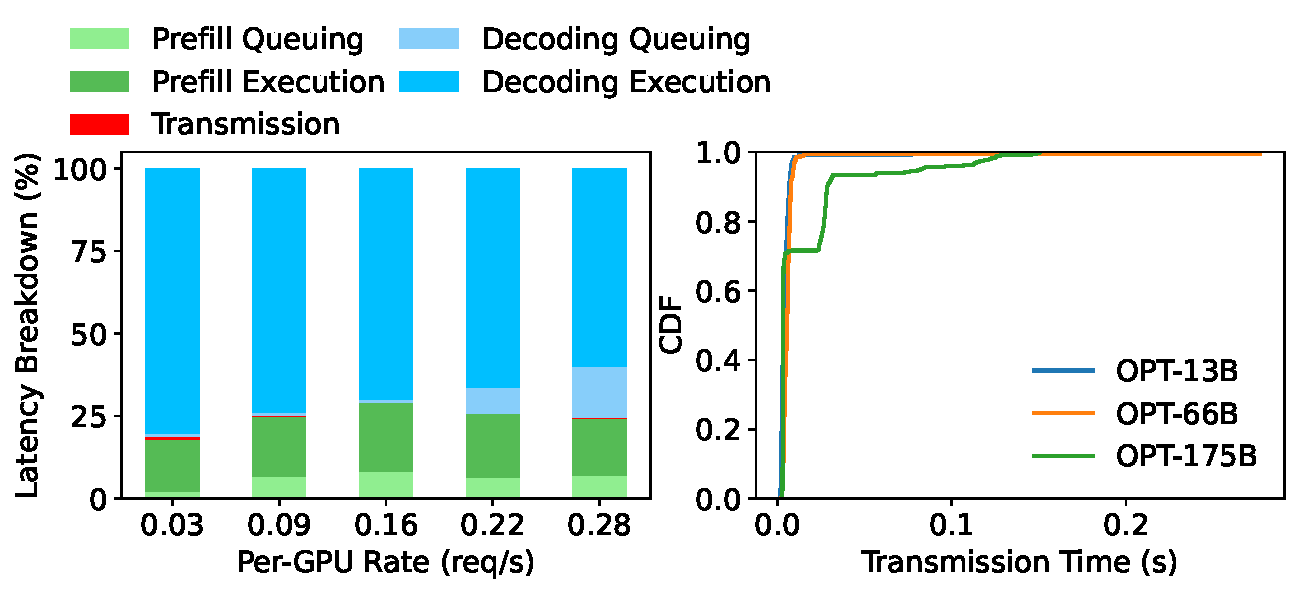
\includegraphics[width=\columnwidth]{figures/evaluation/microbenchmark.pdf}
    \caption{\textit{Left:} Latency breakdown when serving OPT-175B on ShareGPT dataset with \sys. \textit{Right:} The CDF function of KV Cache transmission time for three OPT models.}
    \vspace{-4mm}
    \label{fig:overhead}
\end{figure}

\subsection{Latency Breakdown}
\label{exp:breakdown}

To understand \sys's performance in detail, we make a latency breakdown of the requests in \sys. We divide the processing lifecycle of a request in \sys into five stages: \textit{prefill queuing}, \textit{prefill execution}, \textit{transmission}, \textit{decoding queuing}, and \textit{decoding execution}. The total time consumed by all requests in each stage is then summed up to determine their respective proportions in the system's total execution time. 

Figure~\ref{fig:overhead}\textcolor{green!80!black}{(a)} shows the latency breakdown for the OPT-175B models on the ShareGPT dataset. We chose OPT-175B because the KV Cache transmission is more demanding for larger models. In fact, even for OPT-175B, the KV Cache transmission only accounts for less than 0.1\% of the total latency. Even by examining the CDF of the absolute transmission time shown in Figure~\ref{fig:overhead}\textcolor{green!80!black}{(b)}, we observe that over 95\% of requests experience a delay of less than 30ms, despite our testbed having only limited cross-node bandwidth. This is due to the algorithm described in \S\ref{subsec:practical_placement}, where we require the prefill and decoding instance to maintain the same stage on one machine, enabling the use of intra-node NVLINK bandwidth for transmission, thus significantly reducing transmission delay. 

\begin{table}
\footnotesize
\centering
\begin{tabular}{c|cc|cc}
\toprule
\multirow{2}{*}{\begin{tabular}[c]{@{}c@{}}Rate\\ (req/s)\end{tabular}} & \multicolumn{2}{c|}{vLLM} & \multicolumn{2}{c}{\sys-Low} \\  \cline{2-3} \cline{4-5}
      & Real System & Simulator & Real System & Simulator \\ \midrule
1.0    & 97.0\%      & 96.8\%    & 100.0\%     & 100.0\%    \\
1.5    & 65.5\%      & 65.1\%    & 100.0\%     & 100.0\%    \\
2.0    & 52.8\%      & 51.0\%    & 99.3\%      & 99.3\%    \\
2.5    & 44.9\%      & 46.1\%    & 87.3\%      & 88.3\%    \\
3.0    & 36.7\%      & 38.3\%    & 83.0\%      & 84.1\%    \\
3.5    & 27.8\%      & 28.0\%    & 77.3\%      & 77.0\%    \\
4.0    & 23.6\%      & 24.1\%    & 70.0\%      & 68.9\%    \\
\bottomrule
\end{tabular}
\vspace{-2mm}
\caption{Comparison of the SLO attainment reported by the simulator and the real system under different rates.}
\vspace{-4mm}
\label{table:simulator_fidelity}
\end{table}

\begin{figure}[!t]
    \centering
    
\includegraphics[width=\columnwidth]{figures/evaluation/ablation.pdf}
    \vspace{-6mm}
    \caption{Ablation experiments.}
    \vspace{-4mm}
    \label{fig:ablation}
\end{figure}


\subsection{Ablation Studies}
\label{exp:ablation}
We study the effectiveness of the two key innovations in \sys: disaggregation and the placement searching algorithm. In \S\ref{exp:end_to_end}, we choose the default parallelism setting for vLLM following its original paper~\cite{vllm}. So we implement "vLLM++" which enumerates different parallelism strategies and chooses the best. For \sys, We also compare the placement found by Alg.~\ref{alg:low-affinity-placement} (\sys-Low) with the one found by Alg.~\ref{alg:optimal-placement} (\sys-High) which has fewer searching constraints and assumes high cross-node bandwidth. Since vLLM does not support inter-op parallelism and our physical testbed does not have high cross-node bandwidth, we use simulation for this experiment.

\parabf{Simulator accuracy.} Noticing that DNN model execution~\cite{gujarati2020serving} has high predictability, even under parallel settings~\cite{li2023alpaserve, alpa}.
We study the accuracy of the simulator in Tab.~\ref{table:simulator_fidelity}. For "vLLM" and "\sys-Low", we compare the SLO attainment reported by the simulator and by real runs on our testbed under different rates. The error is less than 2\% in all cases, verifying the accuracy of our simulator.

\parabf{Results.} Figure~\ref{fig:ablation} shows the performance of the four systems when serving OPT-66B on the ShareGPT dataset. "vLLM++" has the same performance as "vLLM" because we find the default parallelism setting (intra-op=4) has the best per-GPU goodput. This further demonstrates the importance of disaggregation. The interference between the prefill and decoding phases significantly reduces the potential performance improvement through adjusting parallelism. In contrast, "DistLLM-High" can achieve further improvements over "DistLLM-Low" because it is not constrained by the deployment constraint that the prefill and decoding instance on one node should share the same model stage. Through disaggregation, we can use tailored parallelism strategies for prefill and decoding instances and optimize their targets without the coupling effects.

\begin{figure}[!t]
    \centering
    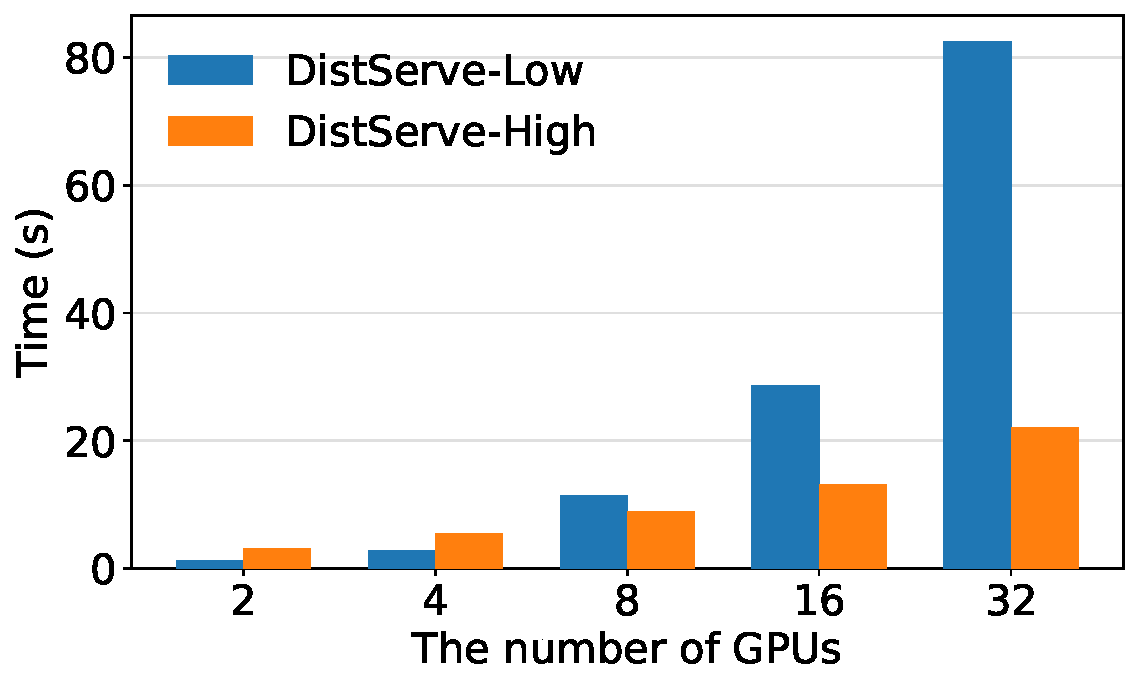
\includegraphics[width=0.8\columnwidth]{figures/evaluation/runtime.pdf}
    \vspace{-3mm}
    \caption{Algorithm Running Time}
    \label{fig:runtime}
    \vspace{-5mm}
\end{figure}

\subsection{Algorithm Running Time}
\label{exp:run_time}
Figure~\ref{fig:runtime} shows the running time for Alg.~\ref{alg:optimal-placement} (\sys-Low) and Alg.~\ref{alg:low-affinity-placement} (\sys-High) on an AWS m5d.metal instance with 96 cores as the number of GPUs ($N \times M$) provided to a single instance increases. According to the results, \sys scales well with the number of GPUs and is independent of the model size. This is because the simulator only simulates discrete events and the running time is the same no matter how big the model is. On the other hand, both algorithms are highly parallelizable, as the searches for different parallelism strategies are independent of each other, allowing the execution time of the algorithms to accelerate almost linearly with more CPU cores. 

As the number of GPUs increases, the execution time of "Dist-Low" becomes higher than that of "Dist-High". This is because the search for parallelism strategies for prefill and decoding instances in "Dist-High" is independent and can be parallelized. But for "Dist-Low", due to additional restrictions on deployment, we need to enumerate all the possible intra-node parallelism combinations for prefill and decoding instances. Even so, the execution time of the algorithm is in minutes, and since it only needs to be executed once before each redeployment, this overhead is acceptable.
